\chapter{Differential characterisation of disulfide bonds}

In this section, we describe the inner workings of Dibby, our program for \gls*{db} mapping in protein \gls*{ms} data, and the way it can be used on real-world data. Additionally, we describe the testing procedure that we used to evalute the program. We start by describing the way we acquired the testing data.

\paragraph{Reagents and instrumentation} Trypsin was purchased from Roche, lyso\-syme, bovine serum albumin, and lipase were obtained from Sigma-Aldrich. The used \gls*{lc} setup was RS\gls*{lc} nano Ultimate 3000 (Thermo Scientific), and Orbitrap Fusion Lumos (Thermo Scientific) was employed for \gls*{msms}.

\paragraph{Input data preparation} We have analyzed two proteins, \gls*{lys}, \gls*{lip}. Parts of the analysis were also performed on \gls*{bsa}.\footnote{The methodology would require some additional automatisaton to make a complete analysis of \gls*{bsa} possible. This is a potential direction for future work.}\footnote{The data have been kindly provided by a IOCB mass specrometry research group (lead by J. Cvačka), and have been measured a few years ago without any direct connection to this thesis.} Two samples of each protein have been obtained in separate sample preparation pathways; in the \emph{AT} pathway, the samples have been alkylated without prior reduction, while in the \emph{RAT} pathway, reduction took place before the alkylation. In both cases the alkylation has been done by iodacetamide (IAA), resulting in a covalent addition of a carbamidomethyl group (57.07 Da) onto cysteines without \glspl*{db}; the reduction was achieved by dithiothreitol (DTT). After that, all samples have been fully digested by trypsine, and the resulting peptides were put into a reverse-\gls*{lc} separation column that was directly connected to the mass spectrometer through a nanospray ion source. After the measurement of \gls*{ms}\textsuperscript{1} spectra on a quadrupole, the precursors continued on to be fragmented with \gls*{hcd}\@. The \gls*{ms}\textsuperscript{2} spectra were analysed on an orbitrap analyser. Finally, raw \gls*{ms}\textsuperscript{2} data were exported to mgf files. Additionally, a control dataset has been generated by in-silico digestion and fragmentation of the protein ovalbumin (\gls*{genova}).

\paragraph{Data analysis} Our own program, described in te next section, has been used for \gls*{db} characterisation. We have set it to only use precursor and fragment assignments with an error of 10ppm or lower, limited the precursors to have at most 3 segments, and limited the fragments to be created by at most two bond cleavages.

\section{Dibby, a program for \gls*{db} mapping}

We have developed a command-line Python program called Dibby that aims to automatically determine the positions of \glspl*{db} in a protein. Its input is the sequence of the analysed protein, and the mgf file with the measured \gls*{ms}\textsuperscript{2} data. Dibby analyses the data and creates a visualisation of evidence for every potential \gls*{db}, and produces a file with the processed data, facilitating further manual analysis of the results. To obtain the best results, it is preferable to do a differential analysis based on data from RAT samples, athough Dibby can analyse the AT data by themselves.

Dibby's function can be split into two separate stages: match assignment, and evidence scoring and visualisation. Both of them are described in detail in their separate sections, what follows is a brief summary. The first stage can be further broken down into the following discrete steps (also illustrated on \Cref{fig:pipeline}):

\begin{enumerate}
  \item Dynamically generated peptides are assigned to the precursor masses from the input. The result of this step is a list of \emph{precursors}, which are effectively slices of the input protein with an added information about the number of present \glspl*{db} and amino acid modifications.
  \item \emph{Variants} are generated from every precursor; a variant is also a slice of the original protein, but with concretely specified configuration of \glspl*{db} and cysteine alkylations. A variant is generated for every valid combination of bonds and alkylations in the precurosor; the more cysteines and \glspl*{db} there are in a precursor, the more variants are generated from it.
  \item \emph{Fragments} produced from the variants are assigned to peaks from the respective spectra.
\end{enumerate}

The second stage of the program interprets the data generated by the first stage; the steps are briefly summarised on \Cref{fig:score-calculation}, and can be descibed as:

\begin{enumerate}
  \item Precursor assignments are scored based on their various properties.
  \item Fragment assignemnts are scored, again based on their various properties.
  \item Variants are scored by combining the score of their parent precursor and the scores of their fragments.
  \item The evidence about individual \glspl*{db} or alkylated cysteines being present in a fragment is weighted by the score of the variant from which the fragment comes. After that the evidence from all fragments is aggregated and the results are visualised.
\end{enumerate}


\begin{figure}
  \centering
  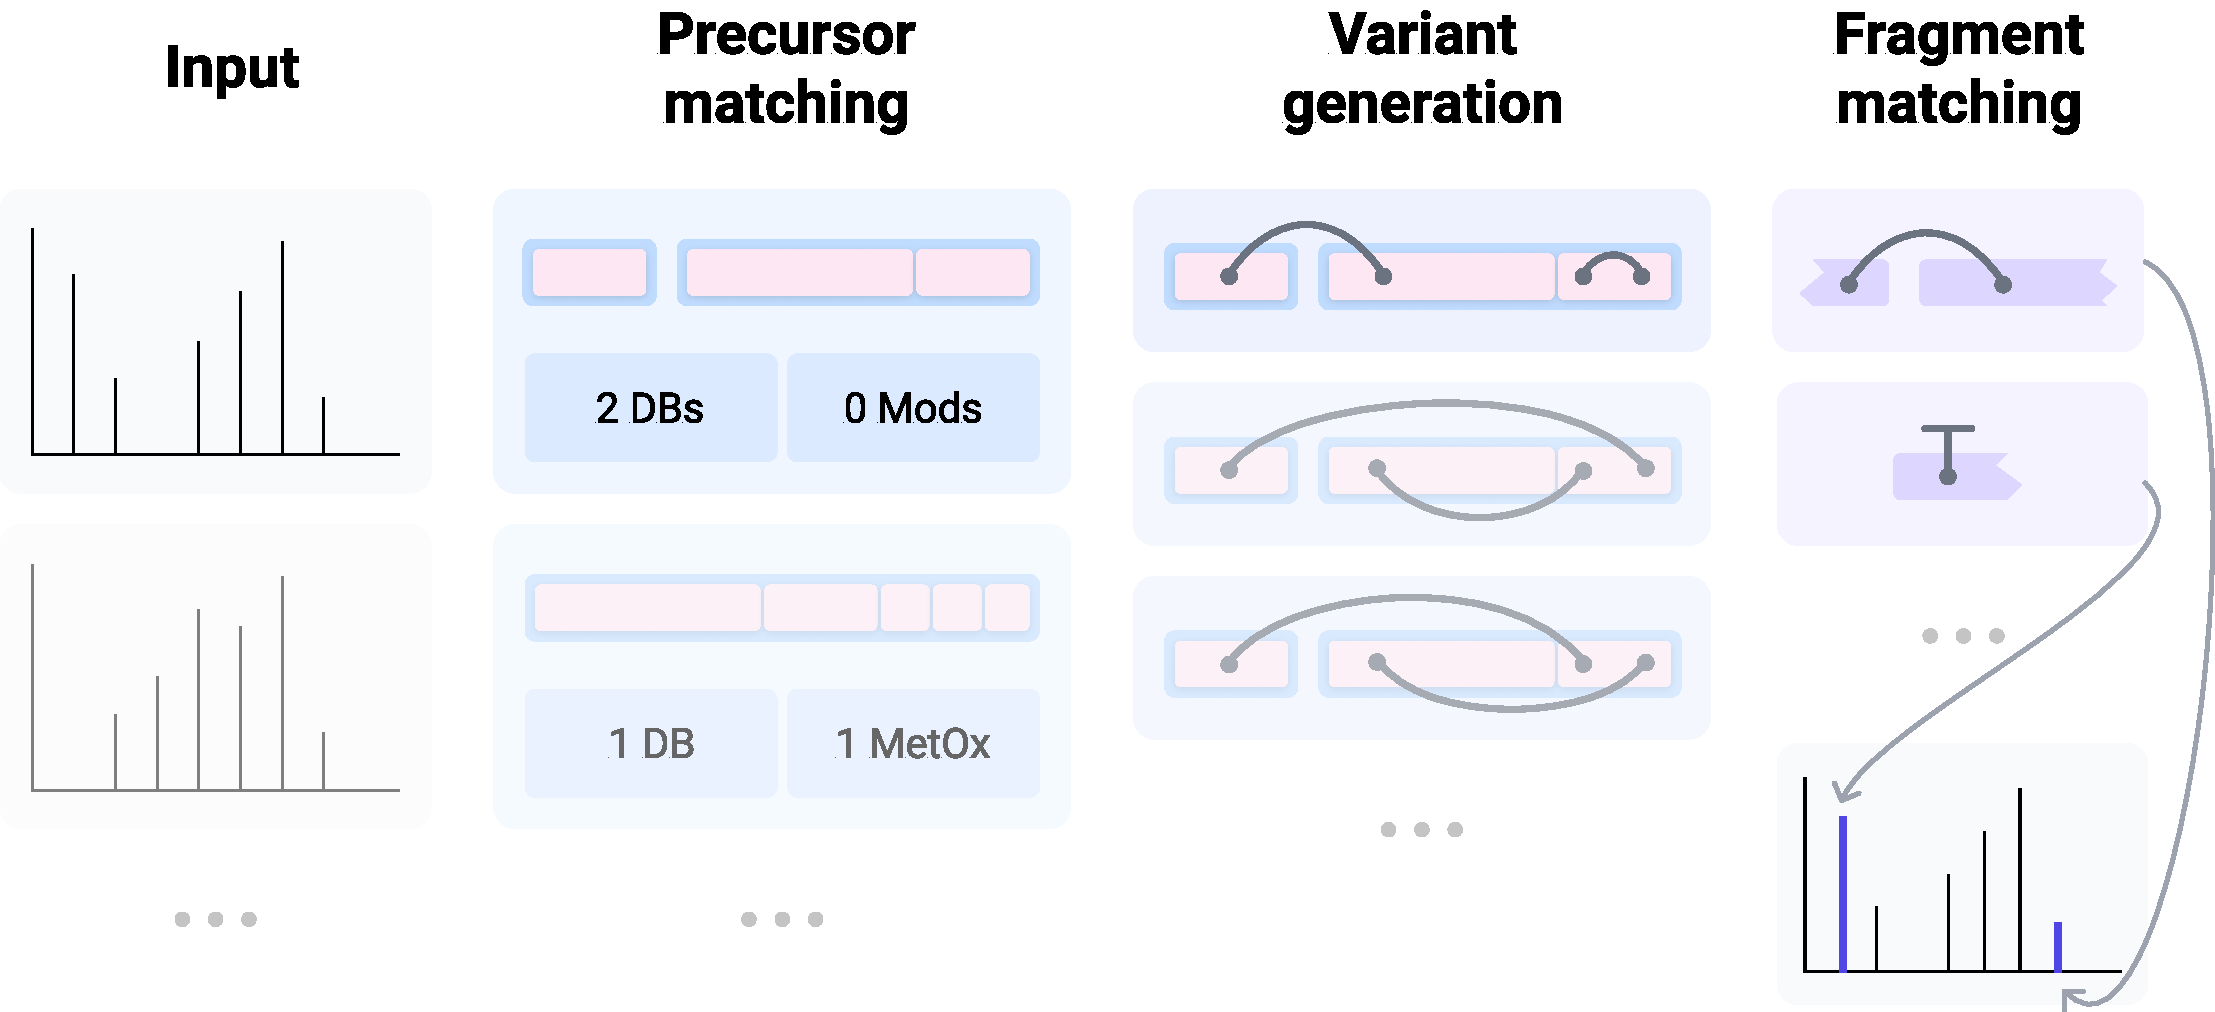
\includegraphics[width=\linewidth]{img/pipeline.pdf}
  \caption{The processing and assignment pipeline in Dibby, not including scoring and visualisation. First, precursors are assigned to the provided spectra, then the precursors are used to generate \emph{variants}, and finally, fragments of the variants are assigned to the peaks in the spectra. Refer to the main text for definitions of each of the terms. Pink bits represent basal peptides resulting from protein digestion, or \emph{tryptides}, and the bigger blue rectangles around them respresent \emph{segments}, longer peptides made of one or more \emph{tryptides}.}\label{fig:pipeline}

\end{figure}

\begin{figure}
  \centering
  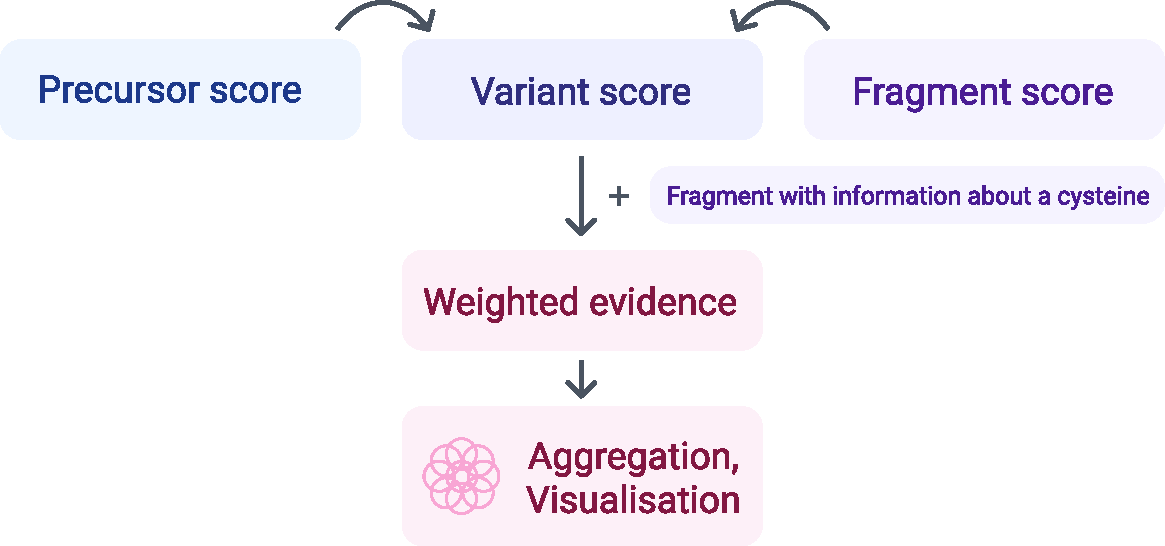
\includegraphics[width=0.75\linewidth]{img/score-calculation.pdf}
  \caption{This figure illustrates how the evidence about \gls*{db} linkage is weighted and aggregated. Our goal is to evalute the evidence for each possible \gls*{db}; the evidence is gathered from the fragment assignments. To forster the quality of the evidence, Dibby tries to weed out false positive assignments by weighting evidence from each fragment by the score of its variant. The variant score is calculated from the precursor score and the score of assigned fragments belonging to the variant.}\label{fig:score-calculation}
\end{figure}


\subsection{Precursor assignment}

At the beginning, the protein undergoes a complete in-silico digestion, producing basal peptides that can not be digested any further; the protease of our choosing was trypsin, so we call these basal peptides \emph{tryptides}. As mentioned in the first chapter (\Cref{sec:trypsin}), a protease can sometimes miss a cleavage point, resulting in a peptide chain that is made from two (or more) contiguous basal tryptides. We call a chain of one or more tryptides a \emph{segment}. Due to the presence of \glspl*{db} in our samples, a \emph{precursor} is made out of one or more segments connected with interpeptide \glspl*{db}\footnote{There can be additional \glspl*{db} connecting a segment to another segment, and there can also be intrasegment \glspl*{db}.}.


From the point of view of this stage of the algorithm, it matters not where the individual \glspl*{db} are located, because the differen \emph{variants} are not distiguishable on the basis of precursor mass. Thus, for each precursor that it managed to assign to a spectrum, the output of the precusor matching algorithm only includes the following information:

\begin{itemize}
  \item  Which segments are present in the precursor.
  \item How many \glspl*{db} there are in the precursor.\footnote{The number of \glspl*{db} is always at least the number of segments minus 1.}, and, by extension, how many alkylated cysteines there are --- every cysteine that does not partake in a bond is considered alkylated. Notice the algorithm does not say anything about \emph{where} the bonds or alkylations are.
  \item How many other amino acid modifications, for example methionine oxidations, are there? The set of available modifications is configurable, and these modifictaions are treated the same as ``variable'' modifications are treated in other software.
\end{itemize}


The precursor is built iteratively segment by segment, and the individual segments are built tryptide by tryptide, from left to right. First of all, given a target mass, the algorithm chooses a beginning of the first segment. After that the \textsc{FindPrec} function iteratively branches out to search the solution space for precursors with a theoretical mass within an error boundary around the target. A pointer to the list of tryptides is kept, and we will call the tryptide that is pointed to in some specific iteration of the function the ``current'' tryptide. In each iteration, each of the following is attempted:

\begin{enumerate}
  \item Combine the \Var{Selected} segments with poteintial modifications and \glspl*{db} in such a way that together they the correct mass, using the \textsc{Combine} function (see \algref{alg:findprec}{alg:findprec:combinations}). \textsc{Combine} implements a divide and conquer algorithm for a modified subset sum problem, in which assignments that are within some error boundary of the target are also considered to be a valid solution.
  \item End the current segment (effectively simulating a protease cleavage just before the current tryptide) and begin a new one that begins on the current tryptide or later. See \algref{alg:findprec}{alg:findprec:end}.
  \item Elongate the current segment by adding the current tryptide to it (see \algref{alg:findprec}{alg:findprec:elongate}).
\end{enumerate}

The fact that the precursors (and their segments) are built strictly from left to right is a simple form of symmetry breaking --- that is, it prevents generating multiple equivalent symmetric solutions. Some further optimizations were added as well, mainly to prevent traversing a branch once we learn it can not provide any more solutions. Finally, the maximum number of segments can be specified, so that precursors containing too many segments are ignored, even though their mass would match the target.


\begin{algorithm}
  \begin{algorithmic}
    \Function{FindPrec}{$I, \mathit{Selected}, \mathit{Mass}, \mathit{Segments}, \mathit{Cys}, \mathit{Open}$}

    % \nb{There is no hanging disulfide bond from previous segments}
    \If{not $\mathit{Open}$}\label{alg:findprec:combinations} \Comment{No hanging \gls*{db} is present}
    \Upd{S}{\textsc{Combine} the segments with some mods to match \Var{TARGET}}
    \EndIf

    \If{$\mathit{Mass}$ is too high, or $i$ is at the end}
    \State return \Var{solutions} \Comment{There are no further solutions in this branch}
    \EndIf

    \If{not \Var{Open}, and $\mathit{Segments} > 0$, and $\mathit{Cys} > 0$}\label{alg:findprec:end}\Comment{Start a new segment}
    \For{every potential start of the next segment from $I + 1$ onward}
    \Upd{S}{\Call{FindPrec}{$\mathit{start}, \mathit{Mass} - \ce{H2}, \mathit{Segments} - 1, \mathit{Cys} - 1, \mathrm{True}$}}
    \EndFor
    \EndIf

    \nb{Elongate the current segment by one tryptide}
    \Decl{t}{the $I$-th tryptide}
    \Decl{open'}{False if this tryptide had any cysteines, otherwise same as \Var{Open}}

    \Upd{S}{\Call{FindPrec}{$I + 1, \mathit{Mass} + t_{mass}, \mathit{Segments}, \mathit{Cys} + t_{cys}, open'$}}\label{alg:findprec:elongate}

    \State return the list \Var{S}
    \EndFunction
  \end{algorithmic}
  \caption{A rough structure precursor matching algorithm, with the respective branching points. Implementation details as well as some of the optimisations were omitted for brevity.}\label{alg:findprec}
\end{algorithm}

\subsection{Fragment assignment}

This part of the program assigns fragments to the peaks from the spectra. The fragments are generated in-silico from the precursors that were assigned by the algorithm from the previous section. There is an additional in-between processing step that generates all possible \emph{variants} that a matched precursor could represent. A \emph{variant} is a set of segments with precisely defined \glspl*{db}, while a precursor only provides information about the number of \glspl*{db}, not their positions. Similarly to how precursors are constructed from crosslinked segments, and the segments from basal tryptides, fragments can also be broken down to smaller pieces; we call these pieces \emph{cuts}. A \emph{cut} is a contiguous slice of one precursor segment.\footnote{The set of interconnected cuts that constitute the fragment forms a connected subgraph in the variant graph.} The fragment is build cut by cut, although this time the cuts are not added from left to right.

To explain the mode of operation of \textsc{FindFrag}, we have to introduce the notion of \emph{pivots}. The algorithm builds a cut residue by residue, until it encouters a cysteine connected by a \gls*{db} to another cysteine in the variant. When the algorihm makes the decision to keep the bond intact, the fragment will definitely have to contain the other cysteine, and possibly some other residues that neighbour it in its segment. The other cysteine is thus added to a list of \emph{pivots}, and when the current cut is ended, the algorithm jumps to a next pivot in the list and builds a new cut around it.

For an outline of the algorithm, see \Cref{alg:fragment}. At the start, a beginning for the first cut of the fragment is chosen from a list of valid beginnings in the variant. The \textsc{FindFrag} function then iteratively explores the solution space by branching out, similarly to \textsc{FindPrec}. The algorithm jumps back and forth between segments, following the directions of \glspl*{db} in the variant, building cuts around pivots, until it either runs out of pivots, runs out of residues in the variant, or until its mass becomes too high. In each iteration, the algorithm attempts to do all of the following:

\begin{enumerate}
  \item Combine the masses of the \Var{Selected} cuts and some of the variable modifications to obtain a fragment with a mass that is within the error boundary around the target mass. In case of a success, add this fragment (that is, this combination of cuts and modifications) to a list of solutions. See \algref{alg:fragment}{alg:fragment:combine}.
  \item If the current residue is a cysteine partaking in a \gls*{db} that we have not seen yet, branch out. In one branch, break the bond, adding assymetric modifications to both of the cysteines, and keep the bond intact in the other branch, adding a new \emph{pivot} to the list of pivots. See \algref{alg:fragment}{alg:fragment:cysteine}.
  \item Elongate the current cut by adding the next residue to it. The ``next residue'' is simply the following residue in the segment in which the current cut is made. If there is no ``next residue'', end this cut, and jump to the next pivot. If there is no pivot to jump to, end this branch of the algorithm. See \algref{alg:fragment}{alg:fragment:elongate}.
  \item End this cut prematurely (in the middle of a segment), that is, simulate a peptide bond dissociation in the precursor. Jump to the next pivot, if there is any, or end this branch of the algorithm. See \algref{alg:fragment}{alg:fragment:end}.
\end{enumerate}

The algorithm keeps track of all residues that are part of the current fragment, in order not to add any residue twice. The maximum number of bond cleavages can be specified, so that fragments that result from more cleavages in the variant are ignored by the algorithm.

On top of what is shown in the pseudocode, Dibby accounts for neutral losses, variable amino acid modifications, multiple number of bond cleavages, asymmetric \gls*{db} cleavages, and a range of potential charges. In total, Dibby is in theory able to identify \emph{all} of the fragments on \Cref{fig:bond-types}.

\begin{algorithm}
  \begin{algorithmic}
    \Function{FragFind}{$I, \mathit{BreaksLeft}, \mathit{Ends}, \mathit{Mass}, \mathit{Pivots}$}

    \Decl{solutions}{an empty list}

    \Decl{can end}{the end would not be premature, or \Var{BreaksLeft} $> 0$}
    \If{\Var{I} is in \Var{Ends}, and also \Var{can end}}

    \If{can \textsc{Combine} the cuts with some mods to match \Var{TARGET}}\label{alg:fragment:combine}
    \Decl{solutions}{the current \Var{solutions} with any of the new ones added}
    \EndIf

    \If{there is some pivot $\mathit{p}$ in $\mathit{Pivots}$}\label{alg:fragment:end}
    \Decl{startrange, endrange}{the valid cut range around \Var{p}}
    \Decl{pivots'}{\Var{pivots} with the pivot \Var{p} removed}
    \Decl{breaks'}{\Var{BreaksLeft}, possibly one less if the end is premature}
    \For{every valid cut start in \Var{startrange}}
    \Decl{S}{\Call{FragFind}{$\mathit{start}, \mathit{breaks'}, \mathit{endrange}, \mathit{Mass}, \mathit{pivots}$}}
    \Decl{solutions}{the current \Var{solutions} concatenated to \Var{S}}
    \EndFor
    \EndIf

    \EndIf

    \If{the \Var{I}-th residue is a cys partaking in a \gls*{db} we have not seen yet}\label{alg:fragment:cysteine}

    \nb{Break the bond...}
    \If{we have some breaks to spare}
    \State add the current cysteine to the broken bond counter, then...
    \Decl{mass'}{the current \Var{Mass} added to the mass of the \Var{I}-th residue}
    \Decl{S}{\Call{FragFind}{$I + 1, \mathit{BreaksLeft} - 1, \mathit{Ends}, \mathit{mass'}, \mathit{pivots}$}}
    \Decl{solutions}{the current \Var{solutions} concatenated to \Var{S}}
    \EndIf
    \nb{...or keep it intact}
    \Decl{pivots'}{add the other end of the bond to \Var{Pivots}}
    \Decl{mass'}{the mass of the bond, $\ce{H2}$, subtracted from \Var{Mass}}
    \Decl{S}{\Call{FragFind}{$I + 1, \mathit{BreaksLeft}, \mathit{Ends}, \mathit{mass'}, \mathit{pivots'}$}}

    \Decl{solutions}{the current \Var{solutions} concatenated to \Var{S}}

    \Else
    \nb{Continue elongating this cut}\label{alg:fragment:elongate}
    \Decl{mass'}{the current \Var{Mass} added to the mass of the \Var{I}-th residue}
    \Decl{S}{\Call{FragFind}{$I + 1, \mathit{BreaksLeft}, \mathit{Ends}, \mathit{mass'}, \mathit{pivots}$}}
    \Decl{solutions}{the current \Var{solutions} concatenated to \Var{S}}
    \EndIf
    \State return the list \Var{solutions}
    \EndFunction
  \end{algorithmic}
  \caption{A very high-level overview of the basic functionality of the fragment matching algotihm.}\label{alg:fragment}
\end{algorithm}

\subsection{Precursor scoring and result visualisation}\label{sec:scoring}

As illustrated on \Cref{fig:score-calculation}, a score of the precursor assignment is combined with scores from the fragment assignment to score the variants. Every fragment that contains a cysteine --- either alkylated or as a part of a \gls*{db} --- is treated as evidence for that specific state of that specific cysteine. The evidence from every fragment is weighted by the score of the variant from which the fragment was made, the results are aggregated and visualised. The scoring is vital for proper function of the program (see \Cref{fig:scoring-metric}); otherwise, the many false positives overwhelm the signal from true positives.

\paragraph{Precursor scoring} The score for a precursor \(P\) is computed as \[\textsc{PrecursorScore}(P) = \frac{1}{1 + \mathcal{w}_P \cdot (\mathrm{variants}_P, \mathrm{mc}_P, \mathrm{mass}_P, \mathrm{error}_P)^T},\] where \(\mathcal{w}_P\) is a vector of weights, \(\mathrm{variants}_P\) is the number of different variants that can be generated from \(P\), \(\mathrm{mc}_P\) is the maximum number of missed cleavages among its segments, \(\mathrm{mass}_P\) is its mass, and \(\mathrm{error}_P\) is the ppm error of the assignment. All of these attributes of are normalised before the score is computed. In this thesis we set \(\mathcal{w}_P = (32, 4, 4, 4)\).

\paragraph{Fragment scoring} The score for a fragment \(F\) is computed as \[\textsc{FragmentScore}(F) = \frac{1}{1 + \mathcal{w}_F \cdot (\mathrm{charge}_{F}, \mathrm{mods}_F, \mathrm{error}_F)^T},\] where \(\mathcal{w}:F\) is a vector of weights, \(\mathrm{charge}_F\) is the charge of the fragment, \(\mathrm{mods}_F\) is the total number of its mods (including neutral losses), and \(\mathrm{error}_F\) is the ppm error of the assignment. All of these attributes are normalised before the score is computed. In this thesis we set \(\mathcal{w}_F = (16, 4, 4)\).\footnote{Our values for \(\mathcal{w}_P\) and \(\mathcal{w}_F\) are aiming to reduce the exploitation of the flexibility of the matching system by large precursors and fragments.}

\paragraph{Variant scoring} The score of a variant \(V\) is computed as \begin{align*}
  \textsc{VariantScore}(V) & = \textsc{PrecursorScore}(\mathrm{precursor}_V)                                                        \\
                           & + w_f \cdot \operatorname{median} \set{ \textsc{FragmentScore}(F) \given F \in \mathrm{fragments}_V }.
\end{align*} In this thesis we use \(w_f = 1/2\).

\paragraph{Score aggregation} For every potential \gls*{db} \(B = (u, v)\) the following evidence score is computed  from the assigned fragments, \[\textsc{DBEvidence}(B) = \sum_{\substack{ \text{assigned} \\ \text{fragment } F }} \textsc{VariantScore}(\mathrm{variant}_F) \cdot [B \in \mathrm{bonds}_F], \] where \(\mathrm{bonds}\) is a set of \glspl*{db} that are present in the fragment. Similarly for every cysteine \(C\) an alkylation score is computed, \[\textsc{AlkylationEvidence}(C) = \sum_{\substack{ \text{assigned} \\ \text{fragment } F }} \textsc{VariantScore}(\mathrm{variant}_F) \cdot [C \in \mathrm{alkcys}_F],\] where \(\mathrm{alkcys}\) is a set of alkylated cysteines that are present in the fragment.

\paragraph{Visualisation} The aggregated evidence is plotted independently for each disulfide bond and --- in the case of alkylation --- for each cysteine (for an example, see \Cref{fig:lys}). The evidence for a bond \((u, v)\) is visualised separately in each direction, \(u \to v\) and \(v \to u\). The evidence for the edge \(u \to v\) is normalised in the context of every other bond \(u \to x\), and the evidence for alkylation of the cysteine \(u\). No further interpretation is done to keep the plots as close to the raw assignment data as possible. In addition to those two plots, plots of ground truth data are shown, representing the theoretical true state of the analysed protein. Alkylation evidence is illustrated by a border around the cysteine.

\paragraph{Interpretation} Due to the nature of the visualisation, we say a bond \((x, y)\) has been \emph{identified} if and only if there is plenty of evidence for the \textbf{bidirectional} connection between cysteines \(x\) and \(y\); on the plot, both of the arrows have to be green. For an example of an identified bond see the edges between \((72, 119)\) on \Cref{fig:genova}. If only one of the arrows is green, the bond is \textbf{not confirmed}, because we have stronger evidence of the other cysteine being in a different configuration. For an example of this, see \(381 \to 119\) on the same figure; in this case, the different configuration with stronger evidence is the abovementioned \gls*{db} \((72, 119)\). Further investigations into the data should be made, though, to determine whether this is caused by the algorithm, or due to a mistreatment of the data during measurement.

\paragraph{Utilisation of the AT and RAT results in differential analysis} Evidence plots are generated for the AT and RAT samples. Bonds that produce strong evidence in the RAT data, where in reality there should be no \glspl*{db} present, are deemed to be prone to generating false positives. For an example, see the bond \((75, 114)\) in the top-right-corner plot on \Cref{fig:lys}. We expect the same bond to generate a lot of false positive signal in the AT sample, too. We can thus use the knowledge acquired from the RAT sample to adjust the scoring of the AT sample. Specifically, we would add the bond \((75, 114)\) to a \gls*{db} blacklist that gets checked by the \(\textsc{FragmentScore}\) and \(\textsc{VariantScore}\) scoring functions; they selectively penalise entities that contain the blacklisted \glspl*{db}.